%\setcounter{subsection}{1}
\subsection*{Principe de la méthode de la méthode d'Euler}

Soit $y$ l'unique solution de 
$\begin{cases}
y'(t)=F(t,y(t))\\y(t_0)=y_0
\end{cases}$ avec $(t_0,y_0)$ fixé.

On souhaite obtenir une approximation de la fonction $y$ sur l'intervalle $[a,b]$.

Soit $n\in\N^*$. 

\begin{itemize}\item  On découpe l'intervalle $[a,b]$ en $n$ sous-segments de même longueur $h=\dfrac{b-a}{n}$.
	
	\item On pose:  $t_0=a\quad t_1=t_0+h\quad t_2=t_0+2h\quad \dots \quad t_k=t_0+kh\quad t_n=t_0+nh=b$.
	On part de $t_0$.
	
	\item On approche la portion de courbe entre $t_0$ et $t_1$ par la tangente à la courbe au point d'abscisse $t_0$.
	
	\vskip1cm\begin{minipage}{0.5\linewidth}
		\begin{center}
			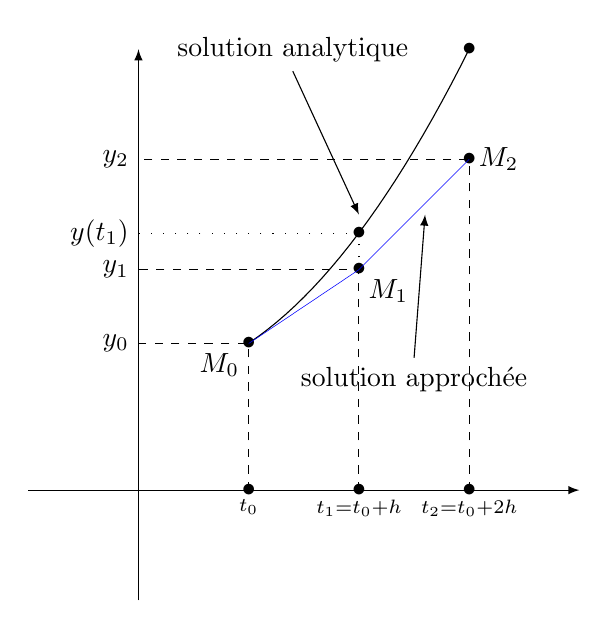
\begin{tikzpicture}[scale=1.4]
				\shorthandoff{:};
				\draw[->,>=latex] (-1,0)--(4,0);
				\draw[->,>=latex] (0,-1)--(0,4);
				\draw[domain=1:3] plot(\x,\x^2/3+1);
				\coordinate (A) at (1,1.33);
				\coordinate (B) at (2,2);
				\coordinate (C) at (3,3);
				\draw[dashed] (1,0)|-(0,1.33)node[left]{$y_0$};
				\draw (1,0) node{$\bullet$}node[below]{$\scriptstyle t_0$};
				\draw[dashed] (2,0)|-(0,2)node[left]{$y_1$};
				\draw (A) node{$\bullet$}node[below left]{$M_0$};
				\draw (B) node{$\bullet$}node[below right]{$M_1$};
				\coordinate (D) at(2,2.33);
				\draw(D)node{$\bullet$};
				\draw[loosely dotted](B)|-(0,2.33);
				\draw(0,2.33)node[left]{$y(t_1)$};
				\draw (C)node{$\bullet$}node[right]{$M_2$};
				\draw (3,4)node{$\bullet$};
				\draw (2,0) node{$\bullet$}node[below]{$\scriptstyle t_1=t_0+h$};
				\draw[dashed] (3,0)|-(0,3)node[left]{$y_2$};
				\draw (3,0) node{$\bullet$}node[below]{$\scriptstyle t_2=t_0+2h$};
				\draw[help lines,color=blue] (A)--(B)--(C);
				\node (solex) at (1.4,4){solution analytique};
				\node (solap) at (2.5,1){solution approchée};
				\draw[->,>=latex] (solex.south)--(2,2.5);
				\draw[->,>=latex] (solap.north)--(2.6,2.5);
			\end{tikzpicture}
		\end{center}
		\shorthandon{:}
	\end{minipage}\begin{minipage}{0.5\linewidth}
		
		Le point $M_1(t_1,y_1)$ appartient à la tangente à la courbe au point $M_0(t_0,y_0)$.\\
		Alors, $y'(t_0) \approx \displaystyle\frac{y_1-y_0}{h}$
		D'où, $y_1=y_0+hy'(t_0)$.\\
		Soit encore, $y_1=y_0+hF(t_0,y_0)$.\\
		$y_1$ est une valeur approchée de la valeur exacte $y(t_1)$.
		
	\end{minipage}
	
	
	%On recommence le procédé à partir du point $M_1(t_1,y_1)$.
	
	\item De manière générale, on pose : $ k\in\{0,\dots,n-1\},\qquad y_{k+1}=y_k+hF(t_k,y_k)$.
	
	Ce qui amène à construire successivement les points $M_k$ de coordonnées $(t_k,y_k)$. La ligne polygonale reliant ces points est alors une approximation de la courbe représentative de la solution.
	
\end{itemize}

\subsection*{Programmation de la méthode }


\question{Considérant l'équation différentielle d'ordre 1 $y'(t)=F(t,y(t))$, écrire en python une fonction \texttt{Euler(F, a, b, y0,n)} d'arguments la fonction $F$, les bornes $a$ et $b$ de l'intervalle d'étude, la condition initiale $y0$ et le nombre d'étapes $n$. Cette fonction renverra une liste de temps et une liste de valeurs approchées par la méthode d'Euler.}
	
\question{Tracer la solution analytique et la solution approchée donnée par la méthode d'Euler pour l'équation différentielle:$$y'(t)+ty(t)=0$$ avec $y(0)=1$. On prendra $a=0$, $b=1$, $n=100$.}
